%test image based on example from Greg Westphal


\documentclass[border=10pt]{standalone}
\usepackage{tikz}
\usetikzlibrary{arrows.meta}
\usetikzlibrary{shapes,decorations}
\tikzset{%
  >={Latex[width=2mm,length=2mm]},
  % Specifications for style of nodes:
            base1/.style = {rectangle, rounded corners, draw=black,
                           minimum width=3cm, minimum height=1cm,
                           text centered, font=\sffamily},
            base2/.style = {ellipse, draw=black,
                           minimum width=.25cm, minimum height=2cm,
                           text centered, font=\sffamily},
       bluebox/.style = {base1, fill=violet!15}, %blue!30
       redbox/.style = {base1, fill=red!30}, %red
       whitebox/.style = {base1, fill = white!30},
       greentank/.style = {base2, fill=green!30}, %green
       process/.style = {base2, minimum width=1cm, fill=gray!30, %orange!15
                           font=\ttfamily},
       tank/.style = {base2, fill = blue!30},
       fueltank/.style = {base2, fill = black!50}
}

% Drawing part, node distance is 1.5 cm and every node
% is prefilled with white background
\begin{document}
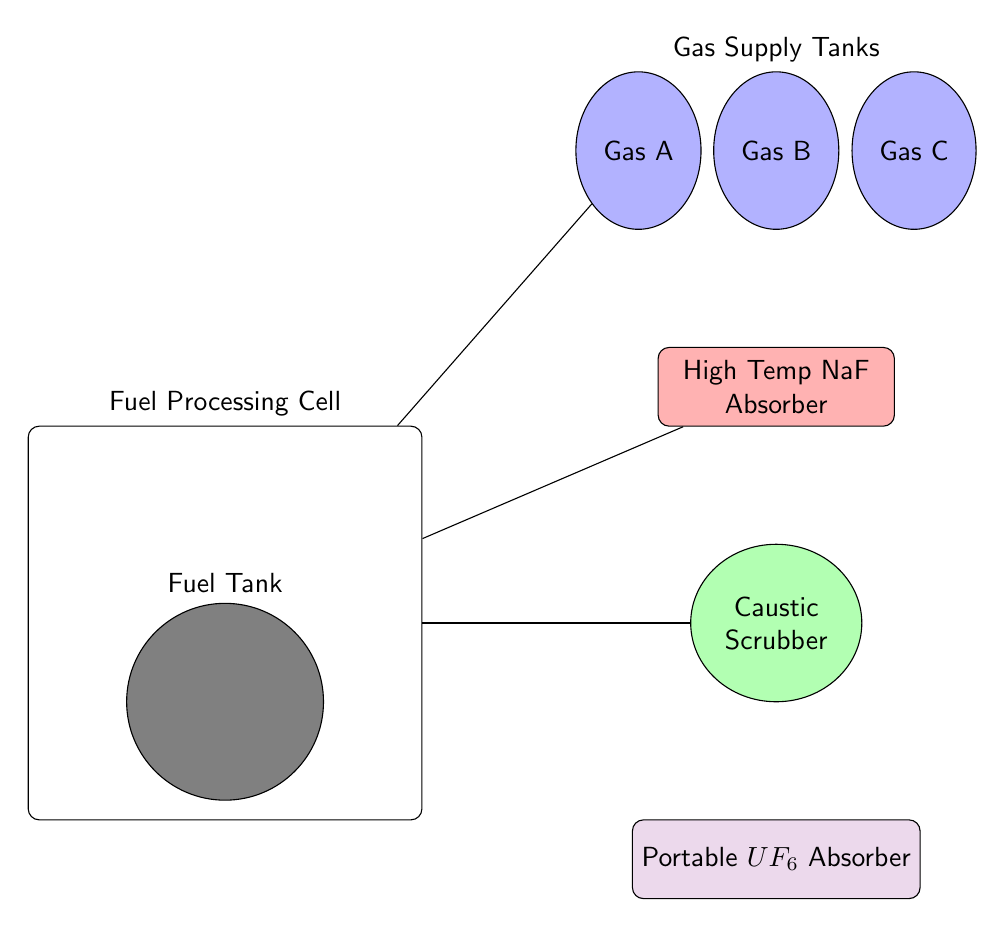
\begin{tikzpicture}[node distance=3cm,
    every node/.style={fill=white, font=\sffamily}, align=center]
  % Specification of nodes (position, etc.)
  \node (gasa)				[tank] {Gas A};
  \node (gasb)				[tank, right of = gasa, xshift = -1.25cm]{Gas B};
  \node (gasc)				[tank, right of = gasb, xshift = -1.25cm]{Gas C};
  \node [above] at (gasb.north){Gas Supply Tanks};
  \node (naabsorber)		[redbox, below of = gasb]{High Temp NaF \\ Absorber};
  \node (scrubber)			[greentank, below of = naabsorber]{Caustic \\ Scrubber};
  \node (ufabsorber)		[bluebox, below of = scrubber]{Portable $UF_6$ Absorber};
  \node (fuelproc)			[whitebox, left of = scrubber, xshift = -4cm, minimum height = 5cm, minimum width = 5cm]{};
  \node [above] at (fuelproc.north) {Fuel Processing Cell};
  \node (fueltank) 			[fueltank,minimum height = 2.5cm,minimum width = 2.5cm, below of = fuelproc, yshift = 2cm]{};
  \node [above] at (fueltank.north){Fuel Tank};
  \draw[-]					(fuelproc) -- (gasa);
  \draw[-]					(fuelproc) -- (naabsorber);
  \draw[-]					(fuelproc) -- (scrubber);
  
  
  \end{tikzpicture}
\end{document}